\documentclass[../diplomski_rad.tex]{subfiles}

\begin{document}


\sloppy

\justifying

U ovom poglavlju opisan je proces razvoja programske potpore za ranije opisani nosivi ugradbeni sustav. 
Programska potpora za korišteni mikrokontroler STM32WB55VGY razvijena je pomoću operacijskog sustava 
za ugradbena računala Zephyr.

Za učitavanje programske potpore na razvijenu pločicu i testiranje sustava korišten je ST-LINK/V2 programator \cite{stm32programator}. 
Progamator se na mikrokontroler spaja putem SWD sučelja (engl. \textit{Serial Wire Debug}). 
Kao razvojno okruženje korišten je Visual Studio Code, a kontrola verzija praćena je sustavom git.

Ovaj integrirani pristup omogućio je efikasno razvijanje i upravljanje programskom podrškom za STM32 mikrokontroler. 
U nastavku će se detaljno opisati proces razvoja, implementacija, te testiranja programske potpore, 
uz naglasak na integraciju sa Zephyr operacijskim sustavom.

\section{Programiranje mrežnog procesora ARM Cortex-M0+}

STMicroelectronics pruža već gotove binarne datoteke \cite{kodovi_M0} koje sadrže kod komunikacijskog stoga. 
Postoje različite verzije komunikacijskog stoga s obzirom na primjenu te je potrebno pronaći odgovarajuću 
binarnu datoteku i učitati ju na jezgru ARM Cortex-M0+.

Binarna datoteka koja je kompatibilna sa operacijskim sustavom Zephyr je \textit{stm32wb5x\_BLE\_HCILayer\_extended\_fw.bin}.
Datoteka je učitana na procesor pomoću programa STM32CubeProgrammer v2.15.0 
koji u sebi ima ugrađenu podršku za ažuriranje koda komunikacijskog stoga. 

\section{Operacijski sustav za rad u stvarnom vremenu Zephyr}

Zephyr je operacijski sustav otvorenog koda (engl. \textit{open-source operating system}) specijaliziran za ugradbene sustave 
i IoT (engl. \textit{Internet of Things}) uređaje.
Glavne karakteristike Zephyra uključuju podršku za različite arhitekture procesora, 
nisku potrošnju energije, brzo pokretanje, podršku za različite komunikacijske protokole kao što su 
Bluetooth, Wi-Fi, LoRaWAN, MQTT, te fleksibilnost u prilagodbi prema specifičnim zahtjevima aplikacija.

\begin{figure}[htb]
    \centering
    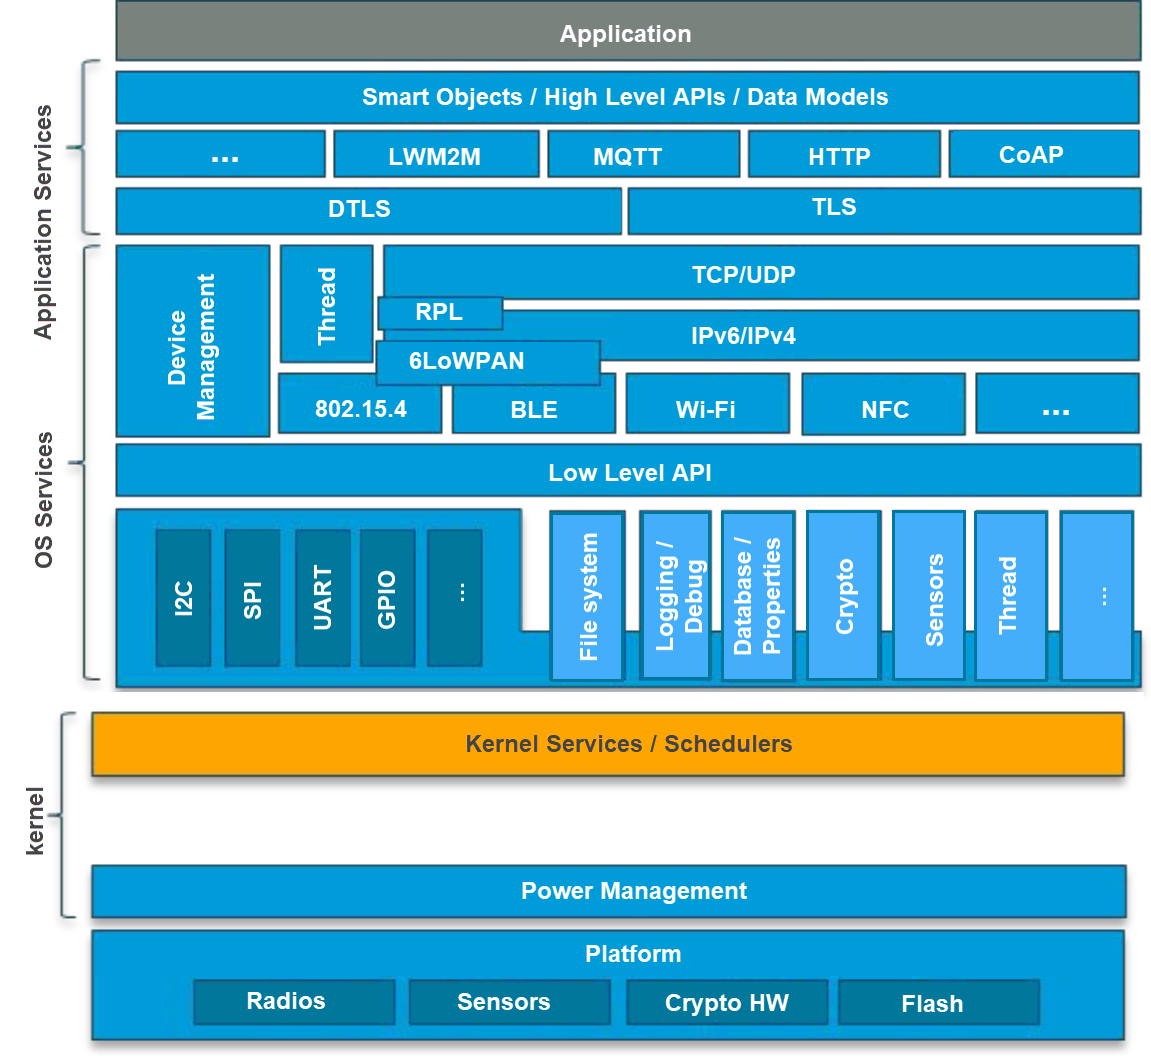
\includegraphics[width=0.75\textwidth]{Figures/zephyr.png} 
    \caption{Arhitektura operacijskog sustava Zephyr \cite{zephyr}}
    \label{slk:zephyr}
\end{figure}

Glavna prednost Zephyra u odnosu na druge operacijske sustave za rad u stvarnom vremenu je njegova 
modularnost i prilagodljivost na različite arhitekture mikrokontrolera. 
Drugim riječima, isti k\^{o}d, uz minimalnu promjenu konfiguracijskih datoteka, možemo koristit na potpuno 
različitim porodicama mikrokontrolera. Iz tog razloga se prilikom razvoja ugradbenog uređaja programska 
potpora može razvijati i dok sklopovlje još nije dostupno.
Također, u sklopu Zepyhr-a već su uključeni brojni upravljački programi za često korištene periferalne 
uređaje i senzore. 
Iz svega navedeno vidljivo je kako korištenje operacijskog sustava Zephyr u konačnici 
znatno ubrzava razvoj uređaja.

Konfiguracija u Zephyr operacijskom sustavu igra ključnu ulogu u prilagodbi ponašanja i funkcionalnosti 
softverskog sustava prema specifičnim potrebama projekta.
Dvije najvažnije datoteke za konfiguraciju Zephyr projekta su \texttt{.conf} te \texttt{.dts} datoteke. 
Važno je naglasiti kako se konfiguracijske datoteke za vrijeme kompajliranja obrađuju i pretvaraju u 
\texttt{\#define} direktive u C kodu. 

DTS (engl. \textit{Device Tree Structure}) je tekstualna datoteka koja
omogućuje opisivanje i konfiguriranje hardverskih svojstava ugradbenog sustava.
Opisuju strukturu i karakteristike hardverskih komponenti poput procesora, 
memorijskih regija, perifernih uređaja, pinout konfiguracija te takta sustava.
Datoteka je pisana u obliku čvorova, gdje svaki čvor predstavlja određenu periferiju. 
Čvorovi imaju parametre pomoću kojih se konfiguriraju korištene periferije.  
Pojedine periferije uključuje se u projekt postavljanjem parametra \texttt{status} na vrijednost \texttt{okay}.
Kroz DTS datoteku Zephyr prepoznaje i uključuje upravljačke programe za konkretno sklopovlje. 
Također, olakšana je migracija projekata na različite platforme jer se konfiguracija može jednostavno 
prilagoditi putem DTS datoteka bez potrebe za izmjenom izvornog koda aplikacije.
Primjer konfiguracije senzora MAX30009 u DTS prikazan je u nastavku teksta, u odsječku koda \ref{lst:dts_max30009}. 

Takt sustava također se konfigurira u DTS datoteci. Svaki izvor signala takta kao i 
RCC (engl. \textit{Reset and Clock Control}) sklop opisani su zasebnim čvorovima. 
RCC sklop služi za upravljanje taktom. Pomoću njega se odabire izvor takta sustava i podešavaju se 
taktovi perifernih sabirnica. 
U razvijenom sustavu kao izvor signala glavnog takta postavljen je takt sa vanjskog visokofrekvencijskog 
oscilatora (engl. \textit{HSE, High-Speed External}) frekvencije 32 MHz. Sve konstante RCC sklopa postavljenje su na 1 
čime je takt svih periferija izjednačen s glavnim taktom sustava.   
\begin{lstlisting}[label={lst:takt},style=CStyle,caption={Konfiguracijska takta sustava},captionpos=b]
    &clk_hse {
        status = "okay";
    };

    &rcc {
        clocks = <&clk_hse>;
        clock-frequency = <DT_FREQ_M(32)>;
        cpu1-prescaler = <1>;
        cpu2-prescaler = <1>;
        ahb4-prescaler = <1>;
        apb1-prescaler = <1>;
        apb2-prescaler = <1>;
    };
\end{lstlisting} 

U \texttt{.conf} datoteci specificiraju se 
konfiguracijske konstante i uključuju se upravljački programi za periferne uređaje. 
Sve naredbe u \texttt{.conf} datoteci započinju prefiksom \texttt{CONFIG}. 
Uključivanje ili isključivanje pojedinih značajki radi se postavljanjem na vrijednosti \texttt{y} ili \texttt{n}.
Konfiguracijska datoteka korištena u ovom projektu prikazana je u odsječku koda \ref{lst:conf}.
\begin{lstlisting}[label={lst:conf},style=CStyle,caption={Konfiguracijska datoteka razvijenog sustava},captionpos=b]
CONFIG_BT=y
CONFIG_BT_HCI=y
CONFIG_BT_CTLR=n
CONFIG_BT_PERIPHERAL=y
CONFIG_BT_DEVICE_NAME="Fluid Track"

CONFIG_GPIO=y
CONFIG_SPI=y
CONFIG_LOG=y
CONFIG_FPU=y

CONFIG_SENSOR=y
CONFIG_ISM330DHCX=y
CONFIG_BME280=y
\end{lstlisting} 

Upravljački programi za senzore BME280 i ISM330DHCX sastavni su dio Zephyr sustava i potrebno ih je uključiti 
pomoću konfiguracijske datoteke. 
Dohvaćanje izmjerenih vrijednosti s tih senzora vrši se generičkim funkcijama za dohvaćanje vrijednosti sa senozra koje 
su također uključene u operacijski sustav Zephyr. 

\section{Opis upravljačkog programa za MAX30009}

Integrirano sučelje za mjerenje bioimpedancije MAX30009 s mikrokontrolerom komunicira SPI 
(engl. \textit{Serial Peripheral Interface, SPI}) protokolom. 
SPI protokol je sinkroni serijski komunikacijski protokol koji omogućava brzu razmjernu podataka između 
mikrokonrolera i perifernih uređaja poput senzora i memorija. 
Podržava istovremeno primanje i slanje podataka uz veliku 
brzinu komunikacije koja doseže nekoliko megabitova u sekundi.
Prvi korak pisanja upravljačkog programa uključivanje je SPI periferije u DTS datoteci:  
\begin{lstlisting}[label={lst:dts_max30009},style=CStyle,caption={Definiranje MAX30009 senzora u DTS-u},captionpos=b]
&spi2 {
    pinctrl-0 = <&spi2_miso_pb14 &spi2_mosi_pb15 
                    &spi2_nss_pb12 &spi2_sck_pb13>;
    pinctrl-names = "default";
    status = "okay";

    gendev: gendev@0 {
            compatible = "vnd,spi-device";
            reg = <0>;
            spi-max-frequency = <1600000>;
            label = "GenDev";
    };	
};
\end{lstlisting} 

Radi lakšeg pisanja upravljačkog programa te njegove portabilnosti na druge sustave za sve SPI funkcije 
napisane su funkcije omotača (engl. \textit{wrapper function}). 
Funckije omotača su funkcije koje služe kao dodatan sloj apstrakcije između aplikacijskog koda i nižih slojeva koda. 
Njihovim korištenjem postignuta je neovisnost aplikacijskog koda o konkretnom sučelju 
SPI funkcija. 
Nalaze se u datoteci \texttt{max30009\_spi\_api.c} te sadrže 
potporu za čitanje i pisanje registra te promjenu pojedine skupine bitova unutar jednog bajta. 

\begin{lstlisting}[label={lst:api_api},style=CStyle,caption={Funkcije omotača SPI komunikacije},captionpos=b]
int max30009_spi_read_reg(uint8_t reg);
int max30009_spi_write_reg(uint8_t reg, uint8_t val);
int max30009_spi_change_reg(uint8_t reg, uint8_t val, uint8_t first_bit, uint8_t num_of_bits);
\end{lstlisting} 

Na početku rada inicijalizira se SPI periferija te se sustav resetira postavljanjem svih registara na tvornički definirano početno stanje. 
Zatim se odabire izvor takta i način rada. Kao način rada odabrana je uzbuda sinusnom strujom 
čija je efektivna vrijednost postaljena je na 64  $\mu$A. 
Zadnji korak inicijalizacije sustava je uključivanje mjernog kanala za mjerenje bioimpedancije.

\begin{figure}[htb]
    \centering
    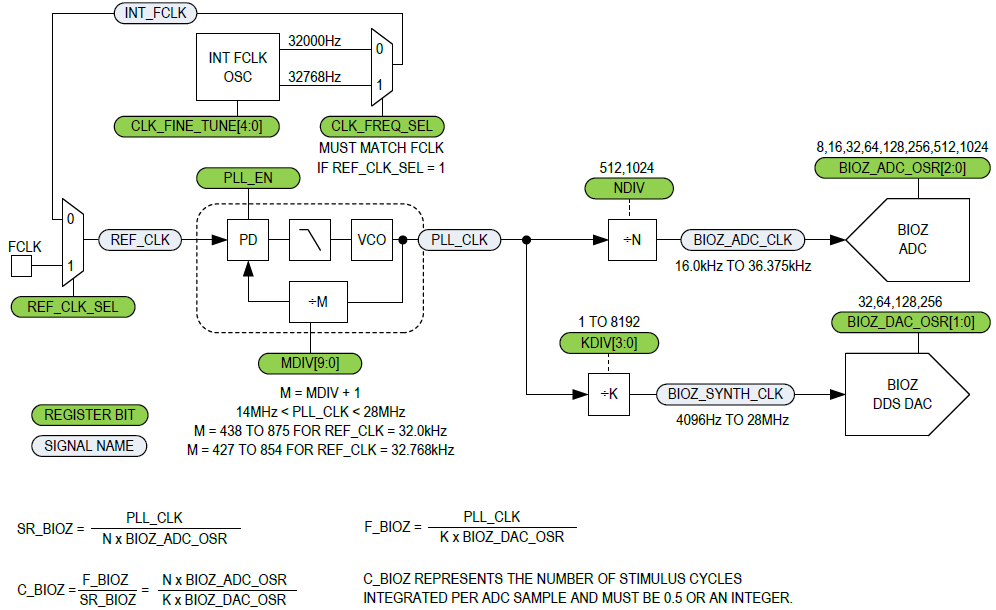
\includegraphics[width=1\textwidth]{Figures/max30009_clock.png} 
    \caption{Vremenski podsustav MAX30009 sustava \cite{max30009_datasheet}}
    \label{slk:max_30009_clock}
\end{figure}

Na slici \ref{slk:max_30009_clock} prikazan je vremenski podsustav MAX30009 integriranog sučelja za mjerenje bioimppedancije.
Kao početni takt sustava odabran je interni oscilator frekvencije 32.768 kHz. Taj se takt dalje vodi na umnoživač frekvencije 
(engl. \textit{PLL, phase-lock loop}) iz kojeg se dobivaju frekvencije između 14 i 28 MHz, u ovisnosti o konstanti \textit{MDIV}. 
Nakon toga se konstantama \textit{KDIV}, \textit{NDIV}, 
\textit{BIOZ\_ADC\_OSR} i \textit{BIOZ\_DAC\_OSR} postavljaju frekvencija uzbudne struje i frekvencija uzorkovanja \cite{max30009_datasheet}.   

Pošto je glavna karakteristika sustava mjerenje bioimpedancije na različitim frekvencijama, upravljački program mora 
omogućavati brzu i laganu promjenu frekvencije uzbudne struje. Zbog toga je stvoren enumeracijki tip podataka koji 
sadrži popis svih korištenih frekvenija i omogućava pisanje generičkih funckija neovisnih o konkretnoj frekvenciji: 
\begin{lstlisting}[label={lst:enumeracija_frekvencija},style=CStyle,caption={Enumeracijski tip podataka za odabir frekvencije rada},captionpos=b]
typedef enum
{
    FREQ_5_kHz,
    FREQ_50_kHz,
    FREQ_100_kHz,
    FREQ_200_kHz,
    
    FREQ_CNT
} max30009_freq_t;
\end{lstlisting} 

Kako bi se promjenila frekvencija sustava potrebno je podesiti ranije spomenute konstante. 
Konstante su upisane u flash memoriju sustava u obliku polja vrijednosti točnim redosljedom kao 
u enumeracijskom tipu podataka za popis korištenih frekvencija što omogućava jednostavnu funkciju 
za promjenu frekvencije prikazanu u odsječku koda \ref{lst:promjena_frekvencije}. 

\begin{lstlisting}[label={lst:promjena_frekvencije},style=CStyle,caption={Funkcija za promjenu frekvenciju sustava},captionpos=b]
void max30009_change_freq(max30009_freq_t freq)
{
    // set dac_osr and adc_osr
    spi_api_change_reg(0x20, dac_osr[freq], 7, 2);
    spi_api_change_reg(0x20, adc_osr[freq], 5, 3);

    // set k,n
    spi_api_change_reg(0x17, k_div[freq], 4, 4);
    spi_api_change_reg(0x17, n_div[freq], 5, 1);

    //set m constant
    spi_api_change_reg(0x17, m_div[freq] & 0x300, 7, 2);         
    spi_api_write_reg(0x18, m_div[freq] & 0xFF);
}
\end{lstlisting}

Kalibracija sustava pokreće se na početku rada te traje nekoliko sekundi.
Za kalibraciju sustava koristi se vanjski precizni otpornik (napisi tu tocne specifikacije). 
Prije početka kalibracije sustav je potrebno konfigurirati na način da se na mjerni kanal povežu 
vanjski kalibracijski pinovi na koji je spojen kalibracijski otpornik. 
Kalibracija se provodi zasebno na svakoj frekvenciji rada sustava, te se kalibracijske konstante pohranjuju 
u memoriju sustava i kasnije koriste za korekciju rezultata mjerenja. 

Za kontrolu MAX30009 senzora stvorena je zasebna dretva. Na početku rada sustava vrši se početna inicijalizacija te 
kalibracija sustava. Nakon toga sustav je spreman za kontinuirano mjerenje. Mjerenje se pokreće i zaustavlja iz 
glavnog programa dvjema funkcijama koje prekidaju i ponovno pokreču dretvu:
\begin{lstlisting}[label={lst:max30009_kontrola},style=CStyle,caption={Funkcije za početak i prekid mjerenja},captionpos=b]
void max30009_start_measuring();
void max30009_stop_measuring();
\end{lstlisting}
U normalnom radu sustava dretva prolazi po svim frekvencijama navedenim u ranije opisanom enumeracijskom tipu podataka. 
Za svaku frekvenciju sustav je potrebno nanovo konfigurirati te pričekati da se sustav utitra na novoj frekvenciji rada. 
Radi toga nakon svake promjene frekvencije prva 3 očitanja su ignorirana i kao rezultat mjerenja uzima se četvrto očitanje. 
Izmjerni podatak ispravlja se u ovisnosti o kalibracijskim konstantama te se nakon toga šalje ispitnom okruženju BLE protokolom. 
Točan format slanja podataka bit će opisan u daljenjem tekstu.

- neki diagram toka bi bio bas zgodan tu!

\section{Bluetooth low energy komunikacija}

Bluetooth Low Energy (BLE) je bežični komunikacijski protokol koji se često koristi u 
nosivim biomedicinskim uređajima zbog svoje energetske učinkovitosti i sposobnosti za prijenos podataka s malom potrošnjom energije.
Mala potrošnja od velike je važnosti kod nosivih uređaja jer time mogu imati manju bateriju i biti lakši te raditi dulje vremensko razdoblje 
bez punjenja ili zamjene baterije. 

U BLE komunikaciji uređaji mogu preuzeti jednu od dvije glavne uloge:
centralni uređaj (engl. \textit{Central}) ili periferni uređaj (engl. \textit{Peripheral}). 
Centralni uređaj inicira vezu i može komunicirati s jednim ili više perifernih uređaja. 
Obično su to uređaji s većom procesorskom snagom i resursima, poput pametnih telefona, tableta ili računala. 
S druge strane, periferni uređaj reklamira svoju prisutnost i čeka da ga centralni uređaj 
pronađe i poveže se s njim. Ovi uređaji su obično s ograničenim resursima, 
poput senzora, pametnih satova ili drugih nosivih uređaja.

\begin{figure}[htb]
    \centering
    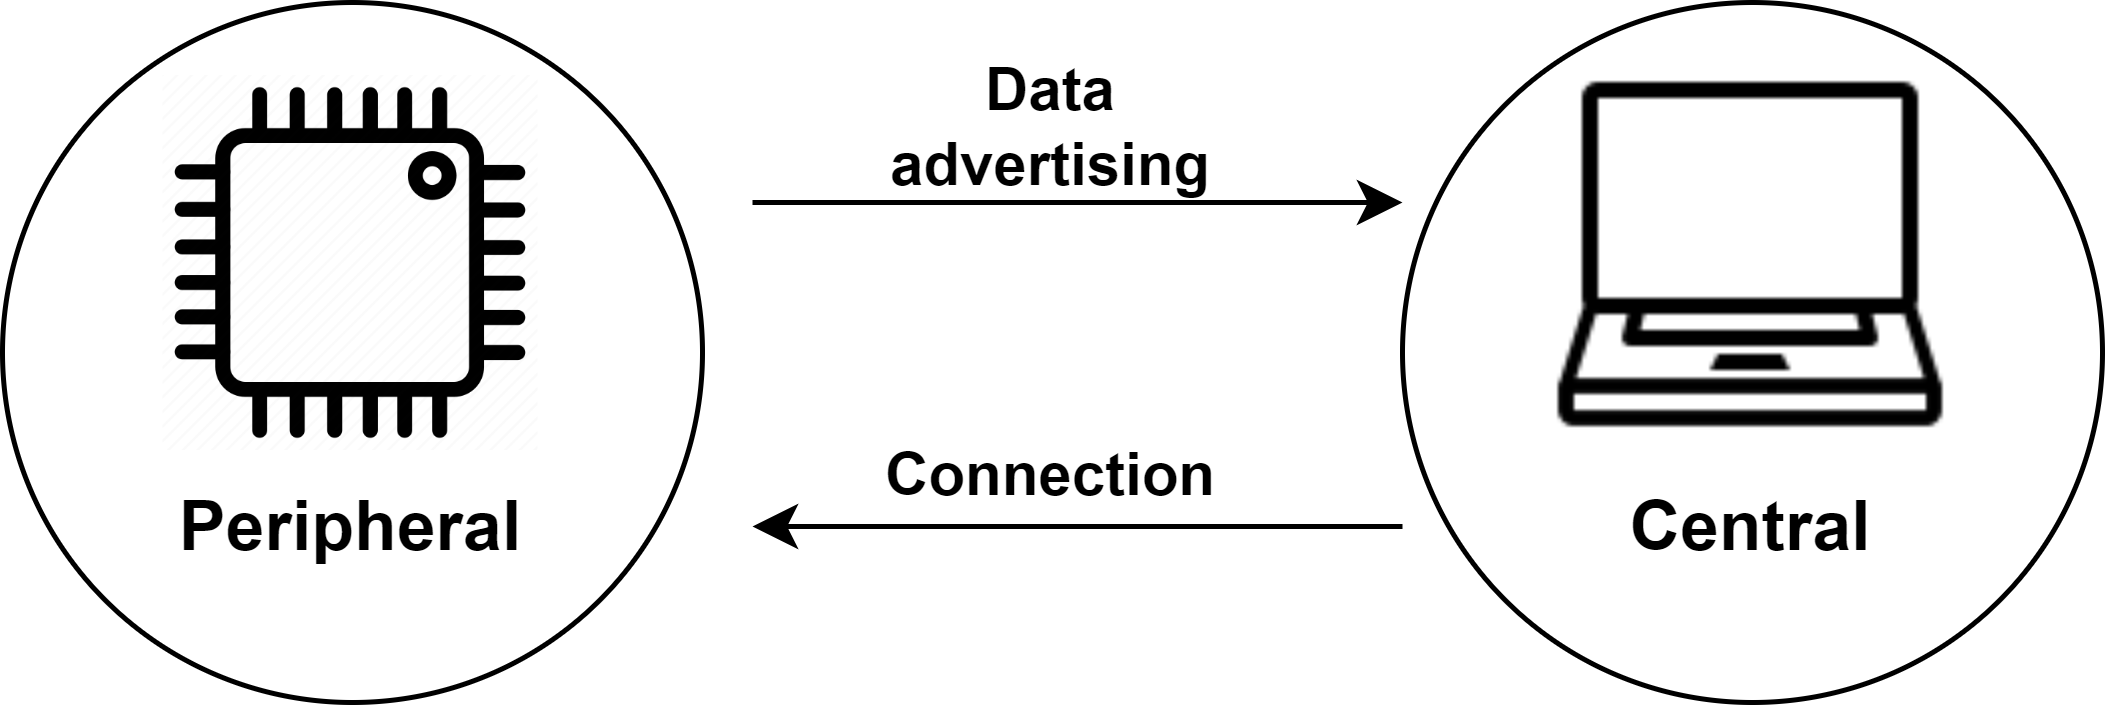
\includegraphics[width=0.75\textwidth]{Figures/ble_role.png} 
    \caption{Uloge uređaja u BLE komunikaciji}
    \label{slk:max_30009_clock}
\end{figure}

Podaci se u BLE komunikaciji organiziraju u servise (engl. \textit{Service}) i karakteristike (engl. \textit{Characteristics}).
Servisi su skupine logički povezanih karakteristika koji definiraju određenu funkcionalnost. 
Karakteristike su najmanje jedinice podataka u BLE komunikaciji. 
Svaka karakteristika ima vrijednost koja se može čitati, pisati ili oboje, ovisno o postavkama. 
Servise i karakteristike prepoznaje se pomoću njihovih UUID (engl. \textit{Universally Unique Identifier}) vrijednosti. 
UUID može biti 16-bitni, 32-bitni ili 128-bitni broj.

Razvijeni nosivi sustav periferni je BLE uređaj konfiguriran kao GATT (engl. \textit{Generic ATTribute Profile}) server 
te pruža jedan servis imena \texttt{BodyFluidMonitoring}. 
Servis \texttt{BodyFluidMonitoring} sastoji se od dvije karakteristike, \texttt{ReceiveCommand} za primanje naredbi i 
\texttt{SendData} za slanje izmjerenih podataka ispitnom okruženju.

\begin{figure}[htb]
    \centering
    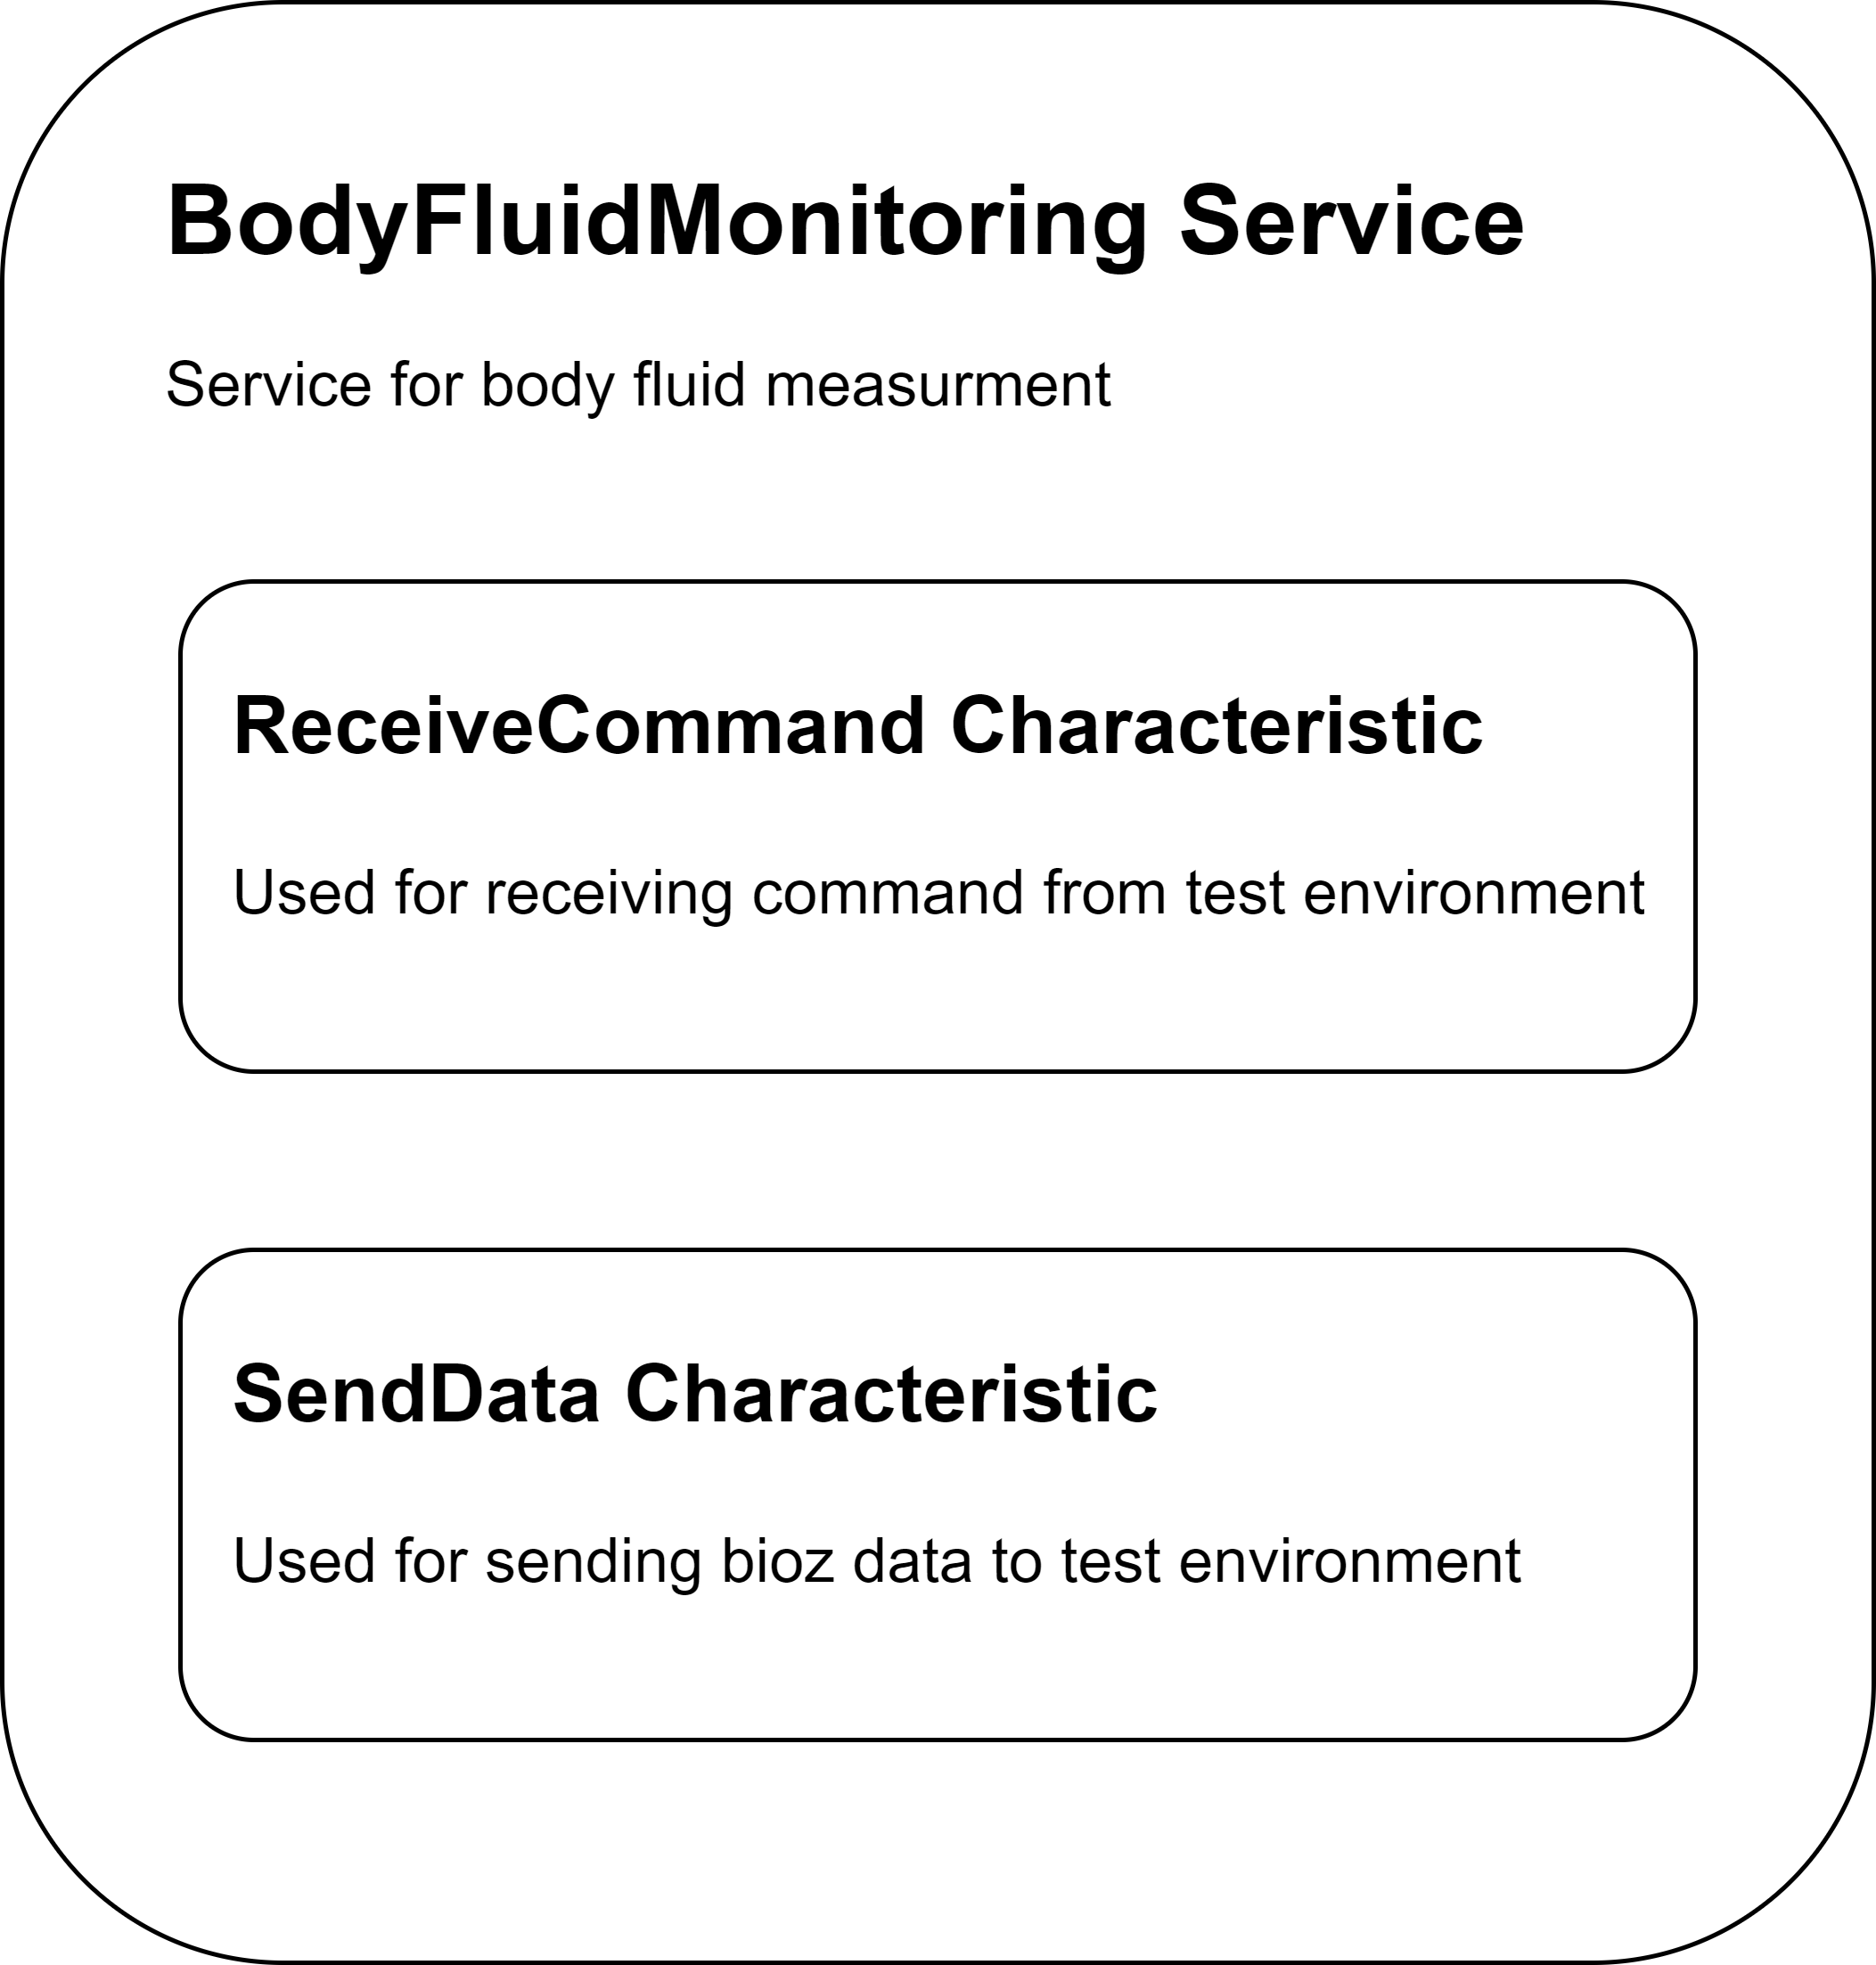
\includegraphics[width=0.5\textwidth]{Figures/ble_service.png} 
    \caption{Konfiguracija GATT servera}
    \label{slk:max_30009_clock}
\end{figure}

Razvijeno aplikacijsko programsko sučelje za kontrolu BLE komunikacije sastoji se od dvije funkcije:
\begin{lstlisting}[label={lst:ble_api},style=CStyle,caption={Programsko sučelje za kontrolu BLE komunikacije},captionpos=b]
void ble_send_data(void *data_to_send, uint8_t data_len);
void ble_init(void (*ble_cmd_handler_callback)(uint8_t));
\end{lstlisting} 

Funkcija \texttt{ble\_init(void (*ble\_cmd\_handler\_callback)(uint8\_t))} inicijalizira BLE periferiju te 
postavlja pokazivač na funkciju koja se poziva kada  \texttt{ReceiveCommand} karakteristika primi naredbu. 
Naredbe su kodirane kao cijeli brojevi te u sustavu postoje dvije, BLE\_CMD\_START i BLE\_CMD\_STOP, kojima se pokreče i zaustavlja mjerenje.  
\begin{lstlisting}[label={lst:ble_received_cmd},style=CStyle,caption={Funkcija koja se poziva kada je primljena naredba},captionpos=b]
static void receive_cmd(uint8_t val)
{
    if(BLE_CMD_START == val)
    {
        max30009_start_measuring();
    }
    else if(BLE_CMD_STOP == val)
    {
        max30009_stop_measuring();
    }
}
\end{lstlisting} 

Razvijeni sustav podatke ispitnom okruženju šalje funkcijom \texttt{ble\_send\_data(void *data\_to\_send, uint8\_t data\_len)} 
kojoj se prosljeđuje pokazivač na podatke koji se šalju i duljinu podataka za slanje. 
Izvršavanjem navedene funkcije ažurira se vrijednost karakteristike \texttt{SendData}.

-slikica ovog

Poruke se šalju u obliku niza znakova čiji format ovisi o senzoru čiji se podatci šalju te je zbog toga uveden dodatan sloj 
apstrakcije između aplikacije i BLE komunikacijskog sučelja.
\begin{lstlisting}[label={lst:ble_send_sensor_data},style=CStyle,caption={Funkcija za slanje rezultata mjerenja sa pojedinog senzora},captionpos=b]
void ble_api_send_sensor_data(void *data_structure, sensor_t sensor);
\end{lstlisting} 
Pri pozivu funkcije za slanje podataka (\ref{lst:ble_send_sensor_data}) kao parametri se zadaju 
pokazivač na podatke senzora i enumeracijski tip \texttt{sensor\_t} koji određuje o kojem senzoru je riječ. 

\begin{lstlisting}[label={lst:sensor_type},style=CStyle,caption={Enumeriacijski tip podataka za odabir senzora},captionpos=b]
typedef enum{
    SENSOR_BIOZ,
    SENSOR_TEMP,
    SENSOR_ACCEL,

    SENSOR_CNT
} sensor_t;
\end{lstlisting} 

Ovaj pristup omogućava generičko korištenje samo jedne funkcije za slanje poruka BLE protokolom, 
neovisno o senzoru čiji podatci se šalju, što u konačnici pojednostavljuje aplikacijski kod. 
Nadalje, u ovinosti o senzoru, primprema se niz znakova u ranije opisanom formatu. 
Zadnji korak u slanju poruke BLE komunikacijskim protokolom je pozivanje ranije opisanih funkcija (\ref{lst:ble_api}) sa 
generiranim nizom znakova.  

Format u kojem se poruke šalju je \texttt{vrijeme;senzor;podatci}. 
Detaljni opis sadržaja poruke razvijenog komunikacijskog protokola prikazan je u tablici \ref{tab:BLE_protokol}. 

\begin{table}[H]
\centering
\begin{tblr}{
    width=1\linewidth,
    cells={valign=m,halign=c},
    row{1}={bg=lightgray,font=\bfseries,rowsep=8pt},
    column{1}={3.5cm},
    column{2}={5cm},
    column{3}={5cm},
    hlines,
    vlines
}
    \hline
    Varijabla & Opis & Vrijednost \\ [0.5ex] 
    \hline\hline
    Vrijeme & Vrijeme proteklo od početka mjerenja izraženo u milisekundama  & Decimalni broj zaokružen na dvije decimale  \\
    Oznaka senzora & Identifikacijska oznaka senzora čiji podatci se šalju  & Cijeli broj u rasponu od 0 do 2, 0 označava bioimpedanciju, 1 temperaturu, a 2 akceleraciju  \\
    Vrijednost & Podaci ovise o senzoru: temperaturni senzor mjeri jednu vrijednost, akcelerometar tri vrijednosti, dok se bioimpedancija izražava s dvije vrijednosti: realnim i imaginarnim dijelom.  & Decimalni brojevi zaokruženi na dvije decimale odvojeni točkom sa zarezom  \\
    \hline
\end{tblr}
\caption{\label{tab:BLE_protokol}Opis dijelova poruke komunikacijskog protokola}
\end{table}

\end{document}